\PassOptionsToPackage{unicode=true}{hyperref} % options for packages loaded elsewhere
\PassOptionsToPackage{hyphens}{url}
%
\documentclass[
  american,
  ignorenonframetext,
]{beamer}
\usepackage{pgfpages}
\setbeamertemplate{caption}[numbered]
\setbeamertemplate{caption label separator}{: }
\setbeamercolor{caption name}{fg=normal text.fg}
\beamertemplatenavigationsymbolsempty
%\setbeameroption{show notes on second screen=right}
% Prevent slide breaks in the middle of a paragraph:
\widowpenalties 1 10000
\raggedbottom
\usepackage{lmodern}
\usepackage{amssymb,amsmath}
\usepackage{ifxetex,ifluatex}
\ifnum 0\ifxetex 1\fi\ifluatex 1\fi=0 % if pdftex
  \usepackage[T1]{fontenc}
  \usepackage[utf8]{inputenc}
  \usepackage{textcomp} % provides euro and other symbols
\else % if luatex or xelatex
  \usepackage{unicode-math}
  \defaultfontfeatures{Scale=MatchLowercase}
  \defaultfontfeatures[\rmfamily]{Ligatures=TeX,Scale=1}
\fi
\usetheme[]{UOS}
% use upquote if available, for straight quotes in verbatim environments
\IfFileExists{upquote.sty}{\usepackage{upquote}}{}
\IfFileExists{microtype.sty}{% use microtype if available
  \usepackage[]{microtype}
  \UseMicrotypeSet[protrusion]{basicmath} % disable protrusion for tt fonts
}{}
\makeatletter
\@ifundefined{KOMAClassName}{% if non-KOMA class
  \IfFileExists{parskip.sty}{%
    \usepackage{parskip}
  }{% else
    \setlength{\parindent}{0pt}
    \setlength{\parskip}{6pt plus 2pt minus 1pt}}
}{% if KOMA class
  \KOMAoptions{parskip=half}}
\makeatother
\usepackage{xcolor}
\IfFileExists{xurl.sty}{\usepackage{xurl}}{} % add URL line breaks if available
\IfFileExists{bookmark.sty}{\usepackage{bookmark}}{\usepackage{hyperref}}
\hypersetup{
  pdftitle={Variables, Assignments and If-statements},
  pdfauthor={Julia Wippermann; Robin Horn; Kamran Vatankhah-Barazandeh; Leonard Frommelt},
  pdfborder={0 0 0},
  breaklinks=true}
\urlstyle{same}  % don't use monospace font for urls
\newif\ifbibliography
\usepackage{listings}
\newcommand{\passthrough}[1]{#1}
\lstset{defaultdialect=[5.3]Lua}
\lstset{defaultdialect=[x86masm]Assembler}
\usepackage{longtable,booktabs}
\usepackage{caption}
% These lines are needed to make table captions work with longtable:
\makeatletter
\def\fnum@table{\tablename~\thetable}
\makeatother
\usepackage{graphicx,grffile}
\makeatletter
\def\maxwidth{\ifdim\Gin@nat@width>\linewidth\linewidth\else\Gin@nat@width\fi}
\def\maxheight{\ifdim\Gin@nat@height>\textheight\textheight\else\Gin@nat@height\fi}
\makeatother
% Scale images if necessary, so that they will not overflow the page
% margins by default, and it is still possible to overwrite the defaults
% using explicit options in \includegraphics[width, height, ...]{}
\setkeys{Gin}{width=\maxwidth,height=\maxheight,keepaspectratio}
\setlength{\emergencystretch}{3em}  % prevent overfull lines
\providecommand{\tightlist}{%
  \setlength{\itemsep}{0pt}\setlength{\parskip}{0pt}}
\setcounter{secnumdepth}{-2}

% set default figure placement to htbp
\makeatletter
\def\fps@figure{htbp}
\makeatother

\usepackage{minted}
\newminted{python}{linenos=false}
\newminted[outputcode]{text}{frame=single, framesep=5pt}
\newenvironment{pyexec}[1]{\noindent \textbf{Output: }  #1}{}
\ifnum 0\ifxetex 1\fi=0 % if pdftex or luatex
  \usepackage[shorthands=off,main=american]{babel}
\else % if xetex
  % load polyglossia as late as possible as it *could* call bidi if RTL lang (e.g. Hebrew or Arabic)
  \usepackage{polyglossia}
  \setmainlanguage[variant=american]{english}
\fi

\title{Variables, Assignments and If-statements}
\author[J.~Wip., R.~Horn, K.~Vat.-Bar., L.~From.]{Julia Wippermann \and Robin Horn \and Kamran Vatankhah-Barazandeh \and Leonard Frommelt}
\date{Apr 10, 2019}

\begin{document}
\frame[plain]{\titlepage}

\begin{frame}
  \tableofcontents[hideallsubsections]
\end{frame}

\hypertarget{what-are-variables}{%
\section{What are variables?}\label{what-are-variables}}

\begin{frame}[fragile,fragile]{What is a variable?}
\protect\hypertarget{what-is-a-variable}{}

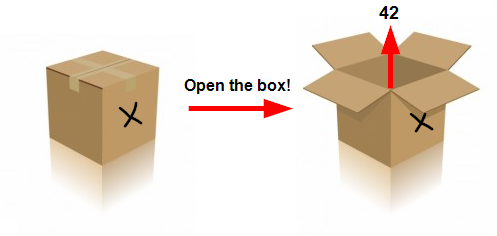
\includegraphics[width=0.6\textwidth,height=\textheight]{02_Variables_Assignments/var_box.png}
MVCodeClub (2019)

\begin{itemize}
\tightlist
\item
  you can ``store'' a value in a variable
\item
  variables are placeholders
\item
  values are the contents
\end{itemize}

\note{A variable is a placeholder for a concept. The value that you can
assign to it, is its realization.

You can think of a variable as a box. The value (that is assigned to it)
is its content.}

\end{frame}

\begin{frame}[fragile,fragile]{Assigning a value to a variable}
\protect\hypertarget{assigning-a-value-to-a-variable}{}

\begin{itemize}
\tightlist
\item
  we use the \texttt{=} operator to assign a value to a variable
  \vspace{2em}
\end{itemize}

\begin{figure}
\centering
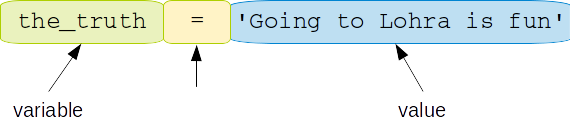
\includegraphics[width=0.9\textwidth,height=\textheight]{02_Variables_Assignments/var_assignment_Lohra.png}
\caption{Variable assignment.}
\end{figure}

\note{
\begin{figure}
\centering
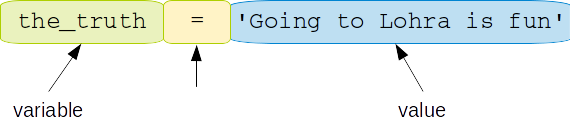
\includegraphics{02_Variables_Assignments/var_assignment_Lohra.png}
\caption{Variable assignment.}
\end{figure}

On the left side of the assignment operator (\texttt{=}) is the
\textbf{variable name} (\texttt{the\_truth}).

On the right side is the \textbf{value} of the variable
(\texttt{\textquotesingle{}Going\ to\ Lohra\ is\ fun!\textquotesingle{}})}

\end{frame}

\begin{frame}[fragile,fragile]{Assigning a value to a variable}
\protect\hypertarget{assigning-a-value-to-a-variable-1}{}

\begin{block}{Caution}

\begingroup\centering

\texttt{=} in code (denoting assignment)

is \textbf{not} the same as

\(=\) in math (denoting equality)

\endgroup

\note{In code, the right side of the equal sign is assigned to the
variable left to the equal sign.

In math, the left and the right side of the equal sign must be equal.}

\end{block}

\end{frame}

\begin{frame}[fragile,fragile]{Variables in Python}
\protect\hypertarget{variables-in-python}{}

\begin{itemize}
\item
  variables are created when they are first assigned
\item
  variables must be assigned before you use them
\end{itemize}

\end{frame}

\begin{frame}[fragile,fragile]{Let's print the variable}
\protect\hypertarget{lets-print-the-variable}{}

\begin{pythoncode}

the_truth = 'Going to Lohra is fun!'

print(the_truth)

\end{pythoncode}

\begin{pyexec}

\begin{outputcode}

Going to Lohra is fun!

\end{outputcode}

\end{pyexec}

\note{\begin{itemize}
\tightlist
\item
  First we assign the string
  \texttt{\textquotesingle{}Going\ to\ Lohra\ is\ fun!\textquotesingle{}}
  to the variable \texttt{the\_truth}.
\item
  To print the content of the variable to the command line, we use the
  print function that you got to know in the last lecture.
\end{itemize}}

\end{frame}

\begin{frame}[fragile,fragile]{Variable assignment}
\protect\hypertarget{variable-assignment}{}

\begin{pythoncode}

the_truth = 'Going to Lohra is fun!'

\end{pythoncode}

\begin{figure}
\centering
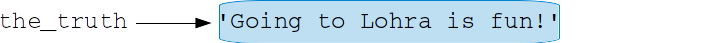
\includegraphics{02_Variables_Assignments/var_assignment_01.png}
\caption{Variable assignment.}
\end{figure}

\end{frame}

\begin{frame}[fragile,fragile]{Assigning a variable to another variable}
\protect\hypertarget{assigning-a-variable-to-another-variable}{}

\begin{pythoncode}

the_truth = 'Going to Lohra is fun!'
fun_fact = the_truth

\end{pythoncode}

\begin{figure}
\centering
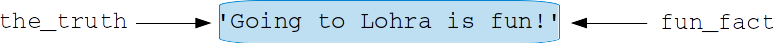
\includegraphics{02_Variables_Assignments/var_assignment_02.png}
\caption{Variable assignment.}
\end{figure}

\end{frame}

\begin{frame}[fragile,fragile]{Variable assignment}
\protect\hypertarget{variable-assignment-1}{}

\begin{pythoncode}

the_truth = 'Going to Lohra is fun!'
fun_fact = the_truth
fun_fact = 'Going to Trash is fun!'

\end{pythoncode}

\begin{figure}
\centering
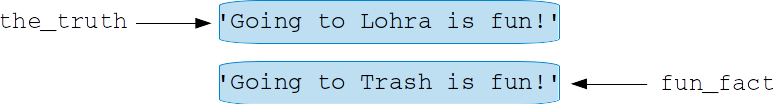
\includegraphics{02_Variables_Assignments/var_assignment_03.png}
\caption{Variable assignment.}
\end{figure}

\end{frame}

\begin{frame}[fragile,fragile]{Variable assignment}
\protect\hypertarget{variable-assignment-2}{}

\begin{pythoncode}

the_truth = 'Going to Lohra is fun!'
fun_fact = the_truth
fun_fact = 'Going to Trash is fun!'
the_truth = 'Learn Python for fun!'

\end{pythoncode}

\begin{figure}
\centering
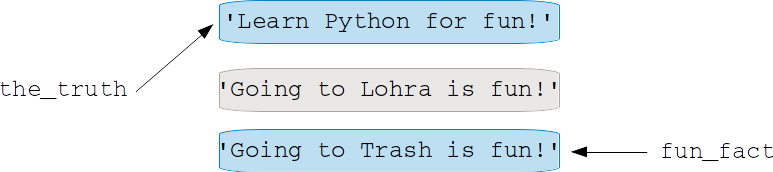
\includegraphics{02_Variables_Assignments/var_assignment_04.png}
\caption{Variable assignment.}
\end{figure}

\end{frame}

\begin{frame}[fragile,fragile]{Recap: string concatenation}
\protect\hypertarget{recap-string-concatenation}{}

\begin{pythoncode}

who = 'Most Coxis think: '
the_truth = 'Going to Lohra is fun!'

# intended output on the command line:
# Most Coxis think: 'Going to Lohra is fun!'

# your code goes here

\end{pythoncode}

\note{\begin{itemize}
\item
  a line in your script that begins with \texttt{\#}, is a comment
\item
  the comment is not executed when you run your script
\item
  strings can be enclosed by single quotes or double quotes
\end{itemize}}

\end{frame}

\begin{frame}[fragile,fragile]{Recap: string concatenation}
\protect\hypertarget{recap-string-concatenation-1}{}

\begin{pythoncode}

who = 'Most Coxis think: '
the_truth = 'Going to Lohra is fun!'

print(who + "'" + the_truth + "'")

\end{pythoncode}

\begin{pyexec}

\begin{outputcode}

Most Coxis think: 'Going to Lohra is fun!'

\end{outputcode}

\end{pyexec}

\note{\begin{itemize}
\item
  we can use the \texttt{+} operator to concatenate two strings
\item
  the comment is not executed when you run your script
\end{itemize}}

\end{frame}

\begin{frame}[fragile,fragile]{print()}
\protect\hypertarget{print}{}

\begin{pythoncode}

answer = 'We are learning'
language = 'Python.'

print(answer + " " + language)
print()
print(answer, language)

\end{pythoncode}

\begin{pyexec}

\begin{outputcode}

We are learning Python.

We are learning Python.

\end{outputcode}

\end{pyexec}

\note{To print the string \texttt{We\ are\ learning\ Python.}, you can
either use string concatenation (\texttt{+}) inside the print function

or

you can separate the variables that you want to print with a comma. Note
that in this case there are spaces between the variables in the output.}

\end{frame}

\begin{frame}[fragile,fragile]{Variable naming rules in Python}
\protect\hypertarget{variable-naming-rules-in-python}{}

\begin{itemize}
\tightlist
\item
  variable names

  \begin{itemize}
  \tightlist
  \item
    can be of any length,
  \item
    can contain uppercase and lowercase letters (A-Z, a-z),
  \item
    digits (0-9),
  \item
    and the underscore character (\_). \vspace{2em}
  \end{itemize}
\end{itemize}

\begin{block}{Caution}

The first character of a variable name cannot be a digit!

\end{block}

\end{frame}

\begin{frame}[fragile,fragile]{Conventions}
\protect\hypertarget{conventions}{}

\begin{itemize}
\tightlist
\item
  choose meaningful variable names
\item
  do not begin variable names with a capital letter

  \begin{itemize}
  \tightlist
  \item
    capital letters are reserved for other things (convention)
  \item
    more about this in the next weeks
  \end{itemize}
\end{itemize}

\end{frame}

\begin{frame}[fragile,fragile]{Conventions}
\protect\hypertarget{conventions-1}{}

\begin{pythoncode}

# do not do this
var_1 = '12.04.2019'
x = '14.04.2019'

print('Lohra is from ' + var_1 + ' to ' + x)

\end{pythoncode}

\begin{pyexec}

\begin{outputcode}

Lohra is from 12.04.2019 to 14.04.2019

\end{outputcode}

\end{pyexec}

\end{frame}

\begin{frame}[fragile,fragile]{Conventions}
\protect\hypertarget{conventions-2}{}

\begin{pythoncode}

# do this
# give your variables descriptive names
start_date = '12.04.2019'
end_date = '14.04.2019'

print('Lohra is from ' +  start_date
      + ' to ' + end_date)

\end{pythoncode}

\begin{pyexec}

\begin{outputcode}

Lohra is from 12.04.2019 to 14.04.2019

\end{outputcode}

\end{pyexec}

\end{frame}

\begin{frame}[fragile,fragile]{}
\protect\hypertarget{section}{}

\begin{itemize}
\item
  make long variables readable by using snake\_case
\item
  snake\_case means that each word is separated by an underscore
  \vspace{1em}

  \begin{pythoncode}

  total_number_of_participants_lohra = 958

  \end{pythoncode}
\end{itemize}

\end{frame}

\hypertarget{what-is-a-data-type}{%
\section{What is a data type?}\label{what-is-a-data-type}}

\begin{frame}[fragile,fragile]{What is a data type?}
\protect\hypertarget{what-is-a-data-type-1}{}

\begin{itemize}
\item
  defines how the value of the variable is stored
\item
  defines which operations are valid for the variable
\end{itemize}

\note{In Python, every value has a data type. There are several data
types in Python. In this lecture, we will learn about strings, integers,
floats and booleans.

These are not all data types. We will get to know a few more in the coming
weeks.
}

\end{frame}

\begin{frame}[fragile,fragile]{Data types in Python}
\protect\hypertarget{data-types-in-python}{}

\begin{itemize}
\item
  the data type of a variable is interpreted based on the value that is
  assigned to the variable
\item
  there is no explicit declaration of a data type for a variable
\item
  use the \texttt{type()} function to check the type of a variable
  \vspace{2em}
\end{itemize}

\begin{longtable}[]{@{}llll@{}}
\toprule
& Type & Description & Example\tabularnewline
\midrule
\endhead
Integer & int & integer of arbitrary magnitude & x = 1\tabularnewline
Float & float & floating-point number & x = 1.0\tabularnewline
String & str & character string & x = `one'\tabularnewline
Boolean & bool & truth value & x = True\tabularnewline
\bottomrule
\end{longtable}

\note{In Python, you do not have to declare the data type of a variable
explicitly. The data type of a variable will be interpreted based on the
value that is assigned to it when you run your code. That means that the
data type of a variable can change while running a script.}

\end{frame}

\begin{frame}[fragile,fragile]{}
\protect\hypertarget{section-1}{}

\begin{pythoncode}

# the variable is a string.
ultimate_answer = 'forty-two'
print('The answer is', ultimate_answer)
print('The type is', type(ultimate_answer))

\end{pythoncode}

\begin{pyexec}

\begin{outputcode}

The answer is forty-two
The type is <class 'str'>

\end{outputcode}

\end{pyexec}

\end{frame}

\begin{frame}[fragile,fragile]{}
\protect\hypertarget{section-2}{}

\begin{pythoncode}

# the variable is an integer
ultimate_answer = 42
print('The answer is', ultimate_answer)
print('The type is', type(ultimate_answer))

\end{pythoncode}

\begin{pyexec}

\begin{outputcode}

The answer is 42
The type is <class 'int'>

\end{outputcode}

\end{pyexec}

\end{frame}

\begin{frame}[fragile,fragile]{}
\protect\hypertarget{section-3}{}

\begin{pythoncode}

# the varibale is a float
ultimate_answer = 42 + 0.0
print('The answer is', ultimate_answer)
print('The type is', type(ultimate_answer))

\end{pythoncode}

\begin{pyexec}

\begin{outputcode}

The answer is 42.0
The type is <class 'float'>

\end{outputcode}

\end{pyexec}

\note{Note that Python does implicit conversion if possible.}

\end{frame}

\begin{frame}[fragile,fragile]{Operations on data types}
\protect\hypertarget{operations-on-data-types}{}

Subtraction is a valid operation on two integers.

\begin{pythoncode}

to_be_paid = 12
given_cash = 15

money = given_cash - to_be_paid
print('The cashier will give you', money, 'Euros.')

\end{pythoncode}

\begin{pyexec}

\begin{outputcode}

The cashier will give you 3 Euros.

\end{outputcode}

\end{pyexec}

\end{frame}

\begin{frame}[fragile,fragile]{Operations on data types}
\protect\hypertarget{operations-on-data-types-1}{}

Subtraction is an invalid operation between an integer and a string.

\begin{pythoncode}

to_be_paid = '12'
given_cash = 15

money = given_cash - to_be_paid

\end{pythoncode}

\begin{pyexec}

\begin{outputcode}

Traceback (most recent call last):
  File "<string>", line 4, in <module>
TypeError: unsupported operand type(s) for -: 'int'
and 'str'

\end{outputcode}

\end{pyexec}

\end{frame}

\begin{frame}[fragile,fragile]{Casting}
\protect\hypertarget{casting}{}

\begin{pythoncode}

to_be_paid = '12'
given_cash = 15

money = given_cash - int(to_be_paid)
print('The cashier will give you', money, 'Euros.')

\end{pythoncode}

\begin{pyexec}

\begin{outputcode}

The cashier will give you 3 Euros.

\end{outputcode}

\end{pyexec}

\note{You can change the type of a variable with a so-called cast
operation.

That only works if Python knows how to convert the previous type into
the other type!

You can cast with functions like:

\begin{itemize}
\tightlist
\item
  int()
\item
  str()
\item
  float()
\end{itemize}}

\end{frame}

\begin{frame}[fragile,fragile]{The Boolean data type - True or False}
\protect\hypertarget{the-boolean-data-type---true-or-false}{}

\textbf{With a Boolean you express truth values:} \vspace{1em}

something is \texttt{True}\\
(which corresponds to \texttt{1})

or

something is \texttt{False}\\
(which corresponds to \texttt{0})

\vspace{2em}

\begin{pythoncode}

  light_on = True
  light_of = False

\end{pythoncode}

\note{\begin{block}{Caution}

Pay attention to the correct spelling of \texttt{True} and
\texttt{False}. Both keywords begin with a capital letter followed by
lower case letters.

\end{block}}

\end{frame}

\begin{frame}[fragile,fragile]{Checking if a statement is True or False}
\protect\hypertarget{checking-if-a-statement-is-true-or-false}{}

\begin{pythoncode}

>>> 10 == 10
True

\end{pythoncode}

\begin{pythoncode}

>>> 1 > 2
False

\end{pythoncode}

\begin{pythoncode}

>>> 2 != 2
False

\end{pythoncode}

\begin{pythoncode}

age = 14
>>>  12 < age < 20
True

\end{pythoncode}

\note{\textbf{Operators for comparisons}

\begin{longtable}[]{@{}llll@{}}
\toprule
Operator & Comparison & \texttt{True} & \texttt{False}\tabularnewline
\midrule
\endhead
\texttt{==} & equal & \texttt{1\ ==\ 1} &
\texttt{5\ ==\ 3}\tabularnewline
\texttt{!=} & not equal & \texttt{2.3\ !=\ 2.313} &
\texttt{5\ !=\ 5}\tabularnewline
\texttt{\textless{}} & less than & \texttt{2.5\ \textless{}\ 9} &
\texttt{4\ \textless{}\ 3}\tabularnewline
\texttt{\textgreater{}} & greater than &
\texttt{2.4\ \textgreater{}\ 2.399} &
\texttt{0.1\ \textgreater{}\ 5}\tabularnewline
\texttt{\textless{}=} & less than or equal & \texttt{3\ \textless{}=\ 3}
& \texttt{4\ \textless{}=\ 3}\tabularnewline
\texttt{\textgreater{}=} & greater than or equal &
\texttt{2.4\ \textgreater{}=\ 2.399} &
\texttt{0\ \textgreater{}=\ 5}\tabularnewline
\bottomrule
\end{longtable}}

\end{frame}

\hypertarget{how-to-write-if-statements}{%
\section{How to write if-statements?}\label{how-to-write-if-statements}}

\begin{frame}[fragile,fragile]{How to make conditional statements?}
\protect\hypertarget{how-to-make-conditional-statements}{}

\begin{figure}
\centering
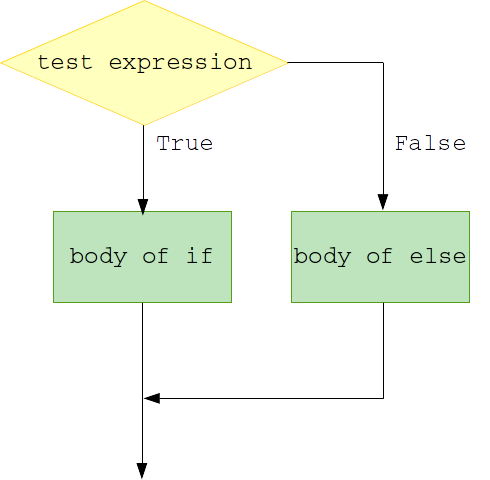
\includegraphics[width=0.5\textwidth,height=\textheight]{02_Variables_Assignments/if_flow_chart.png}
\caption{Control Flow of an if-statement}
\end{figure}

\note{Sometimes you want to execute code depending on whether a
condition is met or not. For this, we can use so called if-statements.

\begin{itemize}
\item
  if the condition after the keyword \texttt{if} evaluates to
  \texttt{True}, the body of the if-statement is executed
\item
  otherwise (\texttt{else}), the body of the else-statement is executed
\end{itemize}}

\end{frame}

\begin{frame}[fragile,fragile]{If - statements}
\protect\hypertarget{if---statements}{}

\begin{pythoncode}

age = 14

if age == 14:
    print('You are 14 years old!')

if 13 <= age <= 19 :
    print('You are a teenager.')
else:
    print('You are not a teenager.')

\end{pythoncode}

\note{\begin{itemize}
\item
  to create an if-statement, we use the keyword \texttt{if}
\item
  same indentation --\textgreater{} block of code
\item
  we indent by using 4 spaces
\end{itemize}}

\end{frame}

\begin{frame}[fragile,fragile]{}
\protect\hypertarget{section-4}{}

\begin{pythoncode}

age = 14

if age == 14:
    print('You are 14 years old!')

if 13 <= age <= 19 :
    print('You are a teenager.')
else:
    print('You are not a teenager.')

\end{pythoncode}

\begin{pyexec}

\begin{outputcode}

You are 14 years old!
You are a teenager.

\end{outputcode}

\end{pyexec}

\end{frame}

\hypertarget{how-to-deal-with-errors}{%
\section{How to deal with errors?}\label{how-to-deal-with-errors}}

\begin{frame}[fragile,fragile]{Errors}
\protect\hypertarget{errors}{}

\begin{alertblock}{Everyone makes mistakes when writing code}
You just need to know how to find them and solve them. $\rightarrow$ Learn
how to understand error messages
\end{alertblock}

\note{Even the most experienced programmers make errors in their code.
When running code, you will also receive error messages and need to
debug your code. Error messages are great as they can often help us to
spot the mistakes more easily and give hints where to start debugging.

\begin{itemize}
\tightlist
\item
  logical mistakes

  \begin{itemize}
  \tightlist
  \item
    your program does not do what it is supposed to do
  \item
    you might notice because you see an unexpected result
  \item
    worse: you trust your output but it was wrongly derived
    --\textgreater{} testing your code can help (more on this in the
    next weeks)
  \end{itemize}
\item
  syntax mistakes

  \begin{itemize}
  \tightlist
  \item
    similar to making an `orthographic mistake'
  \end{itemize}
\end{itemize}

--\textgreater{} understanding error messages is very helpful to spot
and fix the mistakes}

\end{frame}

\begin{frame}[fragile,fragile]{Example error}
\protect\hypertarget{example-error}{}

\begin{pythoncode}

# this is a valid Python statement
goodn8 = 'sleep well'

# this is an invalid Python statement
4u ='for you'

\end{pythoncode}

\note{What is wrong with this piece of code?}

\end{frame}

\begin{frame}[fragile,fragile]{Example traceback}
\protect\hypertarget{example-traceback}{}

\begin{pythoncode}

# this is a valid Python statement
goodn8 = 'sleep well'

# this is an invalid Python statement
4u ='for you'

\end{pythoncode}

\begin{pyexec}

\begin{outputcode}

  File "<string>", line 5
    4u ='for you'
     ^
SyntaxError: invalid syntax

\end{outputcode}

\end{pyexec}

\note{Let's have a look at the traceback:

\begin{itemize}
\item
  what type of error is it?
\item
  what is the problem?
\end{itemize}

Traceback: The sequence of function calls that led to an error.}

\end{frame}

\begin{frame}[fragile,fragile]{Reading the traceback}
\protect\hypertarget{reading-the-traceback}{}

\begin{figure}
\centering
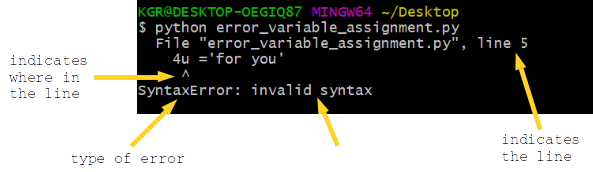
\includegraphics{02_Variables_Assignments/traceback.png}
\caption{Traceback}
\end{figure}

\note{\begin{itemize}
\tightlist
\item
  a variable name must not start with a number
\end{itemize}}

\end{frame}

\begin{frame}[fragile,fragile]{SyntaxError}
\protect\hypertarget{syntaxerror}{}

\begin{itemize}
\item
  your code cannot be interpreted
\item
  similar to making an `orthographic mistake'
\end{itemize}

--\textgreater{} did you only use valid Python statements?

\end{frame}

\begin{frame}[fragile,fragile]{Different types of errors}
\protect\hypertarget{different-types-of-errors}{}

\begin{itemize}
\item
  SyntaxError
\item
  NameError
\item
  ValueError
\item
  TypeError
\end{itemize}

\vspace{3em}

You will learn about these type of errors on the exercise sheet

\note{\textbf{NameError}

\begin{itemize}
\tightlist
\item
  occurs when you use a variable that did not exist before
\end{itemize}

\textbf{ValueError}

\begin{itemize}
\tightlist
\item
  occurs when a function (more about this in the next lecture) is given
  an inappropriate value
\end{itemize}

\textbf{TypeError}

\begin{itemize}
\tightlist
\item
  occurs when a operation is used with inappropriate variable types
\end{itemize}}

\end{frame}

\begin{frame}[fragile,fragile]{Tips for the homework}
\protect\hypertarget{tips-for-the-homework}{}

\begin{itemize}
\item
  to understand what code does

  \begin{itemize}
  \item
    try to run it --\textgreater{} what is the output/error?
  \item
    try to change some variable --\textgreater{} how does the output
    change?
  \end{itemize}
\item
  using a search engine is \textbf{no} cheating!
\item
  collaborate with your peers!
\end{itemize}

\note{Homework

\begin{itemize}
\item
  looks much to do at first, but if you go step by step I am sure, you
  will do great
\item
  biggest hint for almost all the exercises: run the code!!
\item
  play around with code!
\end{itemize}}

\end{frame}

\section*{References}
\addcontentsline{toc}{section}{References}

\begin{frame}{References}

\hypertarget{refs}{}
\leavevmode\hypertarget{ref-mv_code_club2019}{}%
MVCodeClub. 2019. ``Intro to Scratch Stories 6: Rock-Paper-Scissors.''
\url{https://www.mvcode.com/lessons/intro-to-scratch-stories-6-rock-paper-scissors}.

\end{frame}

\end{document}
